\documentclass[../main.tex]{subfiles}
 
Die Festung Vitznau wurde bis 1995 geheim gehalten.

Alle Lichter sind neu LEDs.

Im Gang hat es eine Statue der heiligen Barbara mit Türmen.

In der ganzen Festung hat es Lautsprecher.

Wurde für 35'000 an Vitznau verkauft, plus 8'000 damit sie die Festung so lassen.

Früher war Rauchen drinnen erlaubt.

Bis 1941 nutzten sie einen 2 Takt, 4 Zylinder, 8 Kolben, 80 PS Dieselmotor.

Es hat einen Kohlestofffilter und seit den 50er einen Atomfilter (im Falle einer A-Bombo).

Vor dem Wohn- und Essbereich hat es eine Schleuse mit Dusche.

Beleuchtung war mit Kerzen, wenn sie ausgingen, war zu wenig Sauerstoff in der Luft.

Es hat Thermostate und Luftfeuchtigkeitsmesser in allen Schlafräumen.

Der Kommandant hatte natürlich das beste Schlafzimmer (mit fliessen Wasser, einem richtigen Bett und einem Telefon).

Es hat einen Op-Raum, wurde aber nie benutzt.

Die Instrumente im Op-Raum sind aber immernoch modern.

Sie haben einen Entlausungsaparat benutzt (auf Kopf gesetzt und mit Dämpfen die Läuse umgebracht).

Bis 95 wurde die Festung immer mehr aufgerüstet (sie erhielt sogar eine Dusche).

Die Wohnbereiche, vorallem aber die Krankenräume, sind sehr schön mit Bildern, gelben Wänden und angenehmen Licht gestaltet (Soldaten verbrachten meiste Zeit hier).

Die Lampen sind alle Erbeben (oder Angriff-Beben) sicher mit Sprungfedern.

In der Telefonzentrale hat es einen Swisscom Router :D.

Für den Hotelbetrieb (die Übernachtungen, die sie anbieten), mussten sie Anpassungen machen, wie Geländer bei allen Treppen.

Der Essensraum ist jetzt mit vielen Waffen, Schweizer Flagge und Portrait von Guisan dekoriert.

Das Essen für die Gäste holen sie aus einem Hotel im Dorf und halten es warm.

Der 70-jährige Bunker hält immernoch.

In der Küche konnte für 120 Mann für 2 Monate Essen gelagert werden (Vorallem Kartoffeln).

Überall in der Festung (vorallem im Wohnbereich, wo die Gäste schlafen) hängen Anleitungen zur Festung.

In der Feuerleitstelle haben sie Berechnet wie die Kannone eingestellt werden müssen, um ein bestimmtes Ziel zu treffen.

Zur Berechnung haben sie pro Geschütz ein Blatt, dass sie über eine Karte legen können.

Mittels Testschiessen auf bestimmte Ziele wurden die Daten für das Blatt gesammelt.

Wenn geschossen wurde, wurde das Dorf vorher gewarnt, alle Fenster und Türen zu öffnen (Druckwelle sprengt sonst Glas). 

Nach Schuss, ging ein Soldat durchs Dorf und nahm den Schaden auf, der an Fenstern und Türen geschah.

Telefongeräte sind original von Philips (P68/20 Nr. 221).

Ab den 1950er durfte nicht mehr geschossen werden, da Hotels in Vitznau aufkamen.

Die Festung hat Druckschleusen, damit bei einem Angriff nicht die gesamte Festung zerstört wird.

Im Waffenlager sind unter anderem 14'000 Granaten (Mit Sand gefüllt und ohne Zündstoff).

Im Munitionslager sind unter anderem 40'000 kg Pulver.

Die Festung hat 2 Kannonen, die etwa 10 Schuss/min geben können.

Die Festung hat etwa 4'000 Besucher pro Jahr.

\begin{figure}[b]
    \centering
    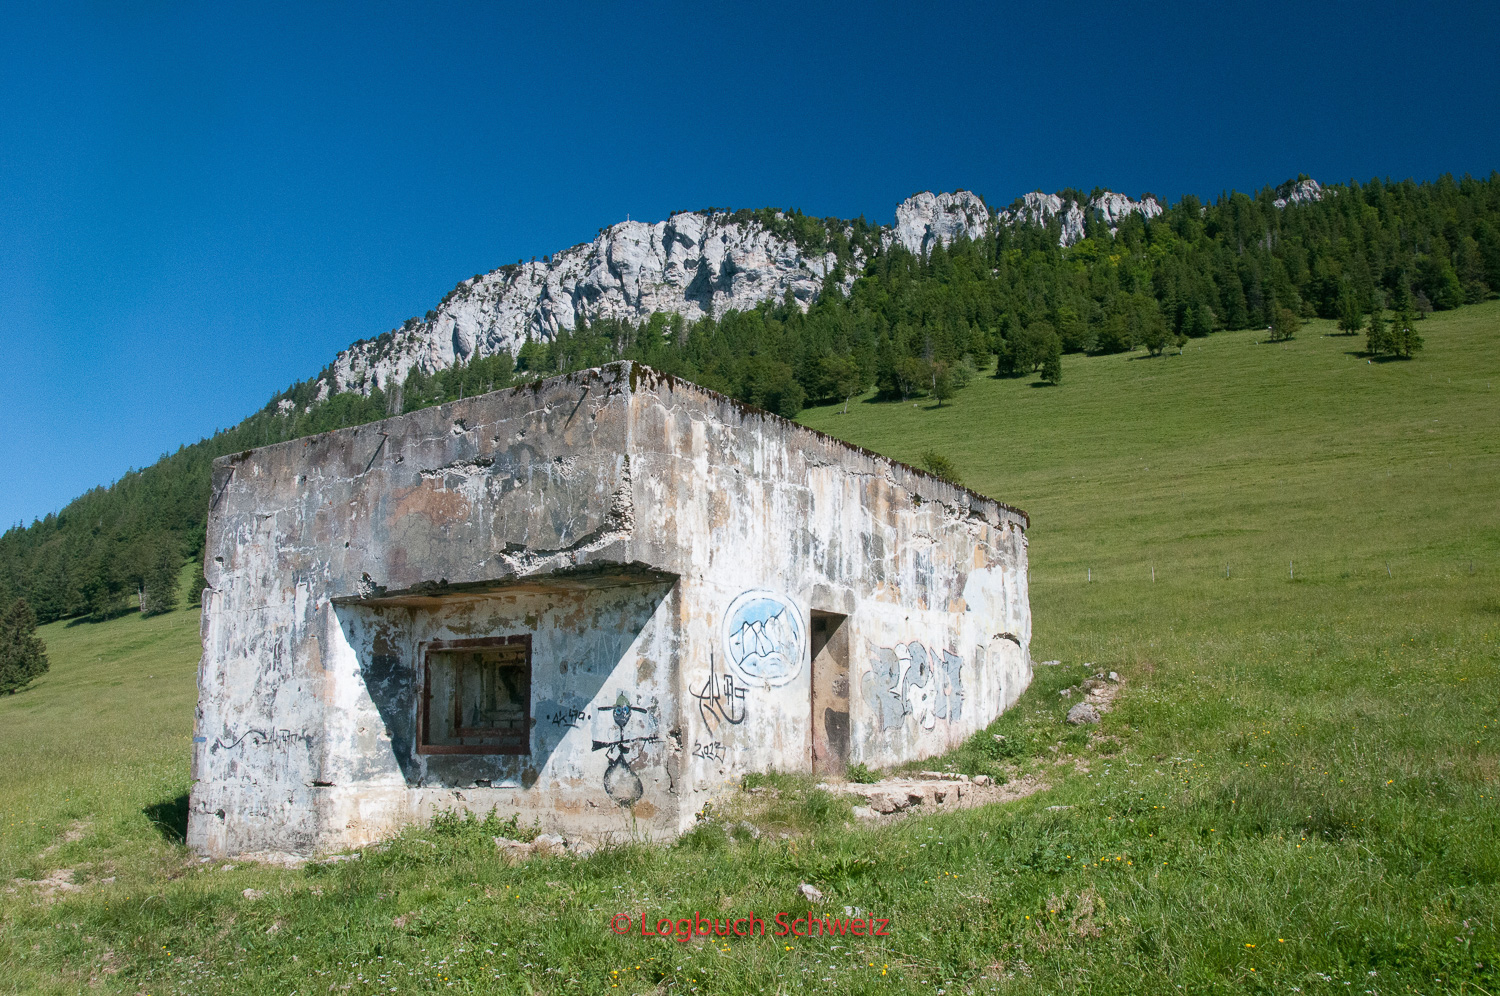
\includegraphics[width=\textwidth]{images/ReduitHangar.jpg}
    \caption{Handgezeichneter Plan der Festung Vitznau kommt noch}
  \end{figure}